
\graphicspath{ {5chapterImplementation/image/} }
\chapter{Implementation}

This chapter will clarify the implementation of the approach present in \ref{Approach}. 
\section{Gray-level conversion and well-composed interpolation}
First of all, the color input images will be transformed into gray level image using its luminance information. Most digital images using the RGB (or sRGB) which use the ITU-R BT.709 primaries. The coefficients defined to calculate the relative luminace from linear RGB components is: $Y = 0.2126R + 0.7152G + 0.0722B$. The formula reflects the spectral sensitivity of human visual perception of brightness: green light contributes the most to the intensity perceived by humans, and blue light the least. Other steps will work on this image. 
\par At first, morphological Laplacian is calculated using a relatively large size structuring element to reduce influences of small components. A morphological gradient will also be calculated to provide information for pruning the tree \textit{a priori}. These output images will be doubled the resolution using a well-composed Interpolation.

\par The topology of the output images are not well-composed and therefor does not provide the self-dual and other topology benefits as said in section \ref{Wellcomposed}. Our method will double the resolution of the image by a well-composed interpolation. This interpolation will add temporary points as in \ref{WllCmpInterpolation} :
\par
\begin{table}
	\centering
	\begin{tabular}{|c|c|c|}
	\hline 
	a & ${(a+b)}/{2}$ & b \\ 
	\hline 
	${(a+c)}/{2}$ & $median(a,b,c,d)$ & ${(b+d)}/{2}$ \\ 
	\hline 
	c & ${(c+d)}/{2}$ & d \\ 
	\hline 

	\end{tabular}
	\caption{Well-composed interpolation} \label{WllCmpInterpolation}
\end{table}

\par
As proved in \cite{geraud.15.ismm}, if added points is calculated by the median of points around them will lead to a self-dual plain map.
\fxnote{interpolate process}


\section{Objects labeling}

\subsection{Labeling by front propagation} \label{labeling}
\par From the well-composed interposed laplacian, we will label all connected components by front propagation. A connected component contain a set of connected pixels that has same sign of Laplacian and zeros that included in that region. As the zeros on the contours is always include in the outer region, we treat connected component in a dual-way i.e this process applied to complement image will give the same result. Thanks for the well-composed interpolation, we can use only one type of connectivity. We chose 4-connectivity to reduce number of neighbors needed to be checked . As there are only 2 type of component (positive and negative one), a region is always surrounded by one other region. With the labeled image, we will present the tree structure with a parent table which tell the parent of each label. The parent of the root will be itself.
\par
Because of large number of component extracted by the Laplacian, we will try to prune the tree at the same time of labeling. Whenever we found a new component, some criteria will be check first to decide if a new label will be spread or continue using the label of that component's parent. These criteria includes average gradient of points on the outer contour and the perimeter of that contour.  
\par
The labeling algorithm is based on front propagation algorithm. At first, an all zeros images is create with the same size like the interpolated Laplacian. Then the output images is read from left to right, top to bottom. When we read point which is not labeled (i.e maintain the null value), a new component is detected and a label will be propagate from that point until all connected points which have same laplacian sign are labeled. If it is not the first point (root component), we will follow points on its boundary to calculate the average gradient and perimeter of this contour and decide if a new label will be use. This contour following algorithm will be presented in \ref{subsec:ContourFollowing}. If the component is small or its gradient is week, we will use its parent's label to mark this component. The label will be propagated in checking its 4 neighbors. If a neighbor is inside the image, still not labeled and having same sign of the region, it will be labeled and the label will continue propagate from that point. The sign agreement can be checked simply by a xor operation between sign of region and sign of that point on the Laplacian. During the labeling process, other information can also be gathered such as the bounding box, area, average gray level of each component. 
\par 
As text must be large enough, if it is not, even the human eye can not recognize them, nor the OCR. Size of a component will be verified by its perimeter and bounding box size. A component is considered noteworthy if:
\begin{itemize} 
	\item $Average_Gradient_on_contour > 30$
	\item $Bounding\_Box\_height >5 pixels $ and $Bounding\_Box\_width>5 pixels $
	\item $\dfrac{Bounding\_Box\_height}{Bounding\_Box\_width} >5 $  
	\item $\dfrac{Bounding\_Box\_width}{Bounding\_Box\_height} >10 $	
\end{itemize}
\par
The pseudo code is presented in Algorithm \ref{alg:labeling}

\begin{algorithm}
\caption{labeling}\label{alg:labeling}
\begin{algorithmic}[1]
\Procedure{Labeling(image,laplacian,gradient)}{}
\State $\textit{output} \gets \text{zeroes }$
\State $ level \gets 1$
\State $ boundingBox \gets image.Domain()$
\For {$\textbf{all } \textit{p}$}
\If {$output(p)$} $\textbf{continue}$
\EndIf
\If {p is the first point}
	\State $current \gets level$
	\State $tree.parent.push\_back(current)$
	\State $tree.color.push\_back(0)$
	\State $tree.area.push\_back(0)$
\Else
	\State $followEdge(p,grad,perimetre,boundingBox)$
	\If{\textit{grad $>$ gradThresHold} \textbf{and} \textit{notSmall(perimetre,boundingBox)}}
		\State $ level \gets level+1$
		\State $ current \gets level$
		\State $tree.parent.push\_back(current)$
		\State $tree.color.push\_back(0)$
		\State $tree.area.push\_back(0)$
		\State $tree.boundingBoxes.push\_back(boundingBox)$		
		\State $newRegionFlag \gets true$		
	\Else
		\State $current \gets output$
		\State $newRegionFlag \gets false$
	\EndIf
\EndIf

\State $output(p) \gets current $.
\State $sign\_flag \gets laplacian(p)>0$.
\State $Queue.push(p)$.

\While {\textit{Queue} \textbf{is not empty}}
	\State p $\gets$ Queue.pop()
	\State $tree.color[current-1] \gets tree.color[current-1] + image(p) $
	\State $tree.area[current-1] \gets tree.area[current-1] + 1$
	\For {$\textbf{all } \textit{neighbor of p} $}
		\If {n \textit{inside} image \textbf{and} output(n) = 0 \textbf{and} sign\_flag = laplacian(n)$ > $0}
			\State $output(n) = current$
			\State $Queue.push(n)$
		\EndIf			
	\EndFor
\EndWhile
\EndFor
\For {$i=0;i<level;i++$}
	\State tree.color[i]=tree.color[i]/tree.area[i];
\EndFor
\State \Return tree, output
\EndProcedure
\end{algorithmic}
\caption{Labeling process to construct the tree}
\end{algorithm}

\subsection{Average gradient on contour calculation} \label{subsec:ContourFollowing}
\par We prune the tree during the labeling process to reduce the calculation cost of reading the image multiple time. By merging nodes which has low contrast with the upper node which means having low gradient in the contour the remain tree only maintain high contrast component. By calculate average gradient of these points, we can decide which node to remove. There are many approach to obtain the contour, for example we can use a dilation follow by a erosion using an element cross as structure element to obtain the contour. But the calculation of erosion and dilation costs. Because the topology is simplified by the well-composed interpolation, which made every component is surround by only one other component, we can apply a simple contour following method to follow its outer contour.
\par As after each label propagation, component which is not yet labeled will remain null and surround by another label. For every new component detected except the first one (root), we will first follow the outer contour of the object to calculate its average gradient. As we read the image from left to right, top to bottom, first point of new region is always the left top most point of that component. 

The algorithm will try to follow the component in clockwise direction so the object will always on the left of each point of the contour. We initialize the starting point is the one on the left of first point of component. There are 8 possible direction of next point to advance (direction are numbered as in \ref{fig:directionToSearch}). The next point must be the one which is labeled and has a non labeled point on its left. The searching order is a semicircle clockwise from last direction plus a semicircle counter-clockwise from last-direction (for example if the last direction is 0, we will check these directions in this order: 0 1 2 3 7 6 5 4). We continue this until reach the starting point. The length and gradient will be gathered during the process. 

\begin{figure}
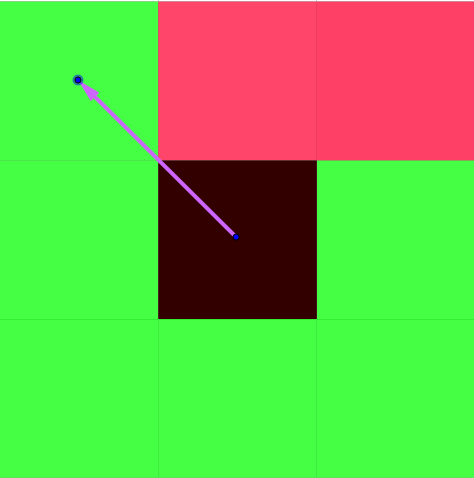
\includegraphics[width=2.5cm]{gradient/7.png}
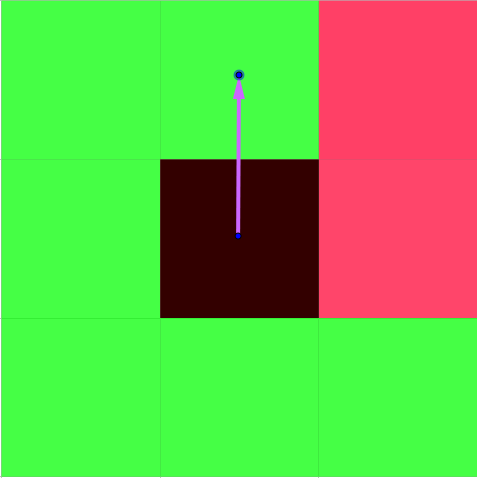
\includegraphics[width=2.5cm]{gradient/8.png}
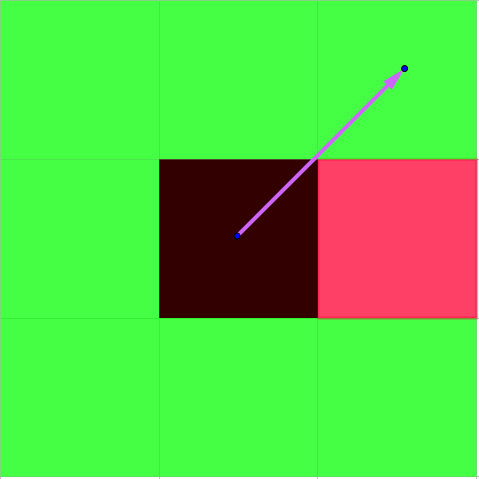
\includegraphics[width=2.5cm]{gradient/1.png}
\centering

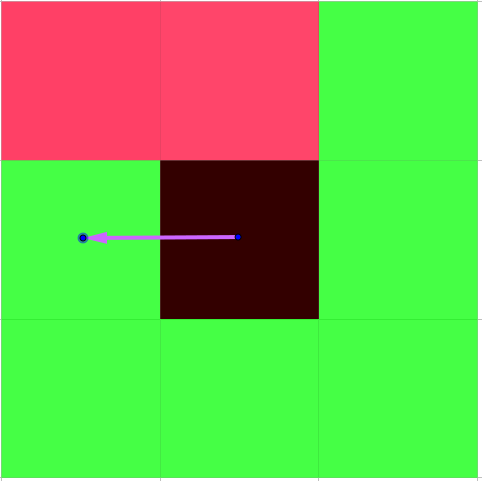
\includegraphics[width=2.5cm]{gradient/6.png}
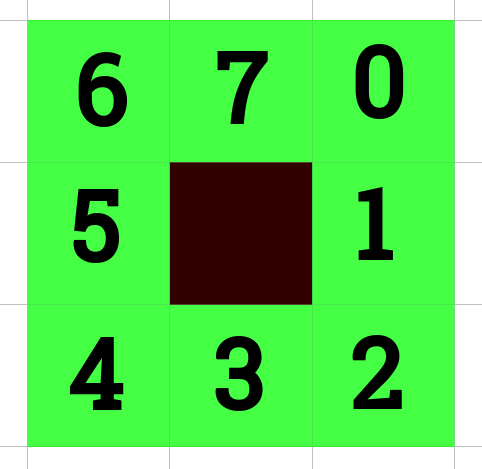
\includegraphics[width=2.5cm]{gradient/c.png}
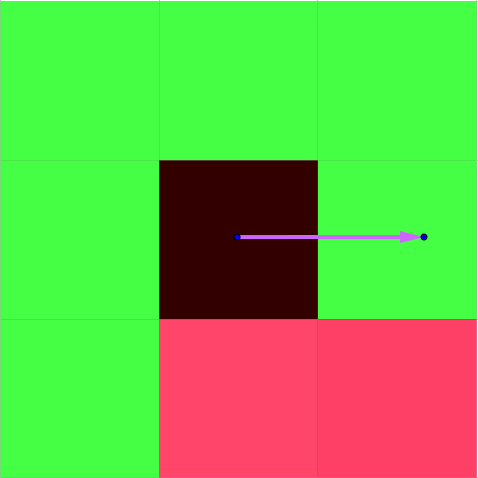
\includegraphics[width=2.5cm]{gradient/2.png}
\centering

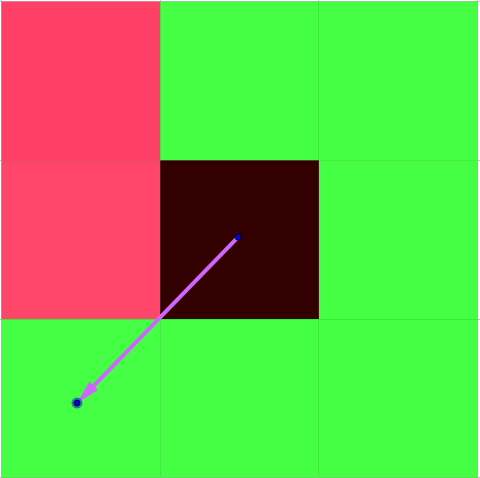
\includegraphics[width=2.5cm]{gradient/5.png}
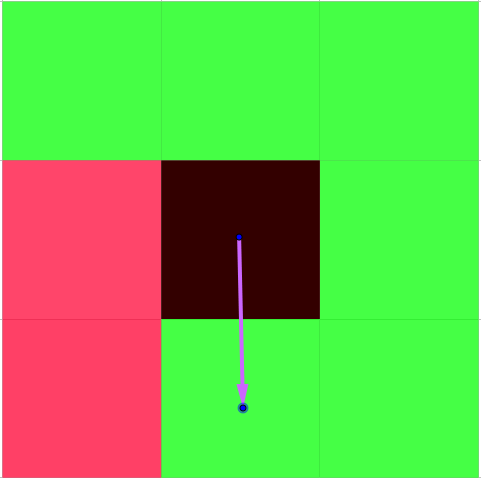
\includegraphics[width=2.5cm]{gradient/4.png}
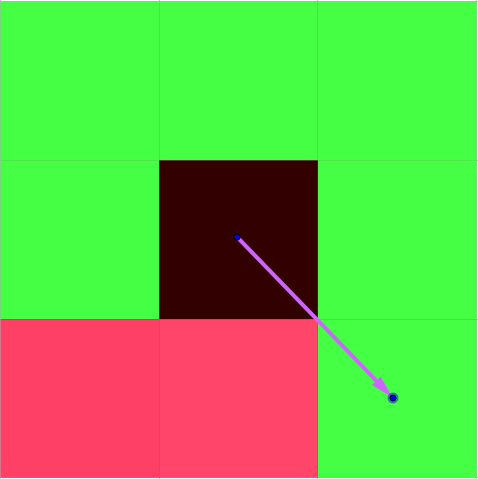
\includegraphics[width=2.5cm]{gradient/3.png}
\centering
\caption{Possible positions of next point on the outer contour}
\label{fig:directionToSearch}
\end{figure}


\begin{algorithm}
\caption{FollowContour}\label{alg:ContourFollowing}
\begin{algorithmic}[1]
\State $iter \gets [0,1,1,1,4,7,7,7]$
\Procedure{FollowContour(p)}{}
\State $np = p$ 
\State $count \gets 0$
\Repeat 
\For{$i=0;i<8;i++$}
	\State $direction \gets (direction + iter[i])$ \textbf{ mod 8}
	\If{$output(np+direction)!=0$ \textbf{ and } $output(np+direction+1)=0$}
		\State $np \gets np+direction$
		\State $grad \gets gradientImage(np)$
		\State $count \gets count+1$
	\EndIf
\EndFor
\Until{$np==p$}
\State $grad\gets grad/count$
\State $perimetre \gets count $
\State \Return (grad,perimeter)
\EndProcedure
\end{algorithmic}
\caption{Contour following process}
\end{algorithm}

\section{Component grouping and bounding box calculation} \label{Grouping}
\par
All the component extracted by the Laplacian will be treated as a character candidate. Of cause they contain a lots of false positive. The labeling process has remove some small or  components .After having the tree structure, we will filtered out components which does not match these criteria:
\begin{itemize} 
	\item $Bounding\_Box\_height >5 pixels $ and $Bounding\_Box\_width>5 pixels $
	\item $\dfrac{Bounding\_Box\_height}{Bounding\_Box\_width} >5 $  
	\item $\dfrac{Bounding\_Box\_width}{Bounding\_Box\_height} >10 $	
	\item $Filling =\dfrac{real\_area}{Bounding\_Box\_height*Bounding\_Box\_width} >0.1$
\end{itemize}
\par
The first three criteria has met since these nodes has been filtered out during the construction of the tree with a single loop. Nodes do not meet the forth criteria will be flagged so they will be transparent during the grouping process. After that, word candidate will be created by grouping remain nodes which have same parent (share the same background) and have relatively small horizontal distance. This value chose is the maximum of height and width of each components. In reading backward the tree table (from leaves to root), we will try to group component with their neighbors. We look at its left and right to find brother node which is in ranges and isn't grouped to another word. For a component found, a double check is done to make sure the other component is in range of this one. This component is grouped in to current word and new component will be search from this one. 
\par
We only interest in word which has more than 2 characters. Only components with similar height is grouped together because characters in the same word do not vary more than 2 of smallest character. We use the generalized Jaccard similarity: 

\begin{center}
    $J(\mathbf{x}, \mathbf{y}) = \dfrac{\sum_i \min(x_i, y_i)}{\sum_i \max(x_i, y_i)}$ 
\end{center}
    
In applying to the height of 2 components, it becomes simple. Components are only grouped if the similarity is greater than 0.5.

\begin{center}
$J(\mathbf{height1},\mathbf{height2}) = \dfrac{min(height1,height2)}{min(height1,height2)} < 0.5$. 
\end{center}


\par We use different strategy to find the neighbors of components. At first, only one searching pointer is use and it situates in the center of that component. We also use 3 different searching pointer, one in the middle, one at 10\% of height from the top and another at 10\% of height from the bottom. 
The pseudo code is present in Algorithm \ref{alg:WordCandidate} for the case of only one searching pointer in the center.

\begin{algorithm}
\caption{Tree prunning and Word candidate grouping}\label{alg:WordCandidate}
\begin{algorithmic}[1]
\Procedure{GetNeighbors}{Component a,component b}
\State \Return $min(a.height,b.height)/max(a.height,b.height)<0.5$
\EndProcedure
\Procedure{GetNeighbors}{Start point \textit{p},searching direction dp}
\State $current \gets image(p)$

\If{direction = left}
	\State move \textit{p} left thisComponent.width/2
\Else
	\State move \textit{p} right thisComponent.width/2
\EndIf

\For{$i=0;i<height;i++$}
\State $p=p+dp$
\If {image does not contain \textit{p}} \textbf{continue} \EndIf
\If {$image(p)=current$} \textbf{continue} \EndIf
\If {$image(p) \neq 1$ \textbf{ and } $ parent(thisComponent) = parent(componentAt(p))$ \textbf{ and } $isSimilar(thisComponent,componentAt(p))$}
	\State \Return image(p)
\Else
	\State $current = image(p)$
\EndIf
\EndFor
\State \Return 0
\EndProcedure
\item[]
\item[]
\Function {JoinWord}{label,box}
	\State $found = 0$
	\State $deja_vu(label)= true$	
	\If {$NeighborRight(label)$ \textbf{ and } $label = NeighborLeft(NeighborRight(label)) $ \textbf{and not } $ deja_vu(NeighborRight(label)) $}
		\State $box.extendToMatch(NeighborRight(label))$
		\State $found \gets found + 1 + JoinWord(NeighborRight(label),box,oldNode)$
	\EndIf
	\If {$NeighborLeft(label)$ \textbf{ and } $label = NeighborRight(NeighborLeft(label))$  \textbf{and not } $ deja_vu(NeighborLeft(label)) $}
		\State $box.extendToMatch(NeighborRight(label))$
		\State $found \gets found + 1 + JoinWord(NeighborRight(label),box,oldNode)$	
	\EndIf
	\State \Return found
\EndFunction
\item[]
\item[]
\Procedure{GetWordCandidate}{a,b}
\For {\textbf{all } label} 
	\If{MatchCharacterCondiditon(label)}
		\State	deja\_vu(label) = true
	\Else
		\State	deja\_vu(label) = false
	\EndIf
\EndFor

\For {\textbf{all } label \textbf{except} root} 
	\State NeighborLeft(label) = GetNeighbors(label.center, leftPointer)
	\State NeighborRight(label) = GetNeighbors(label.center, rightPointer)
\EndFor

\For {\textbf{all } label backward \textbf{except} root} 
	\State new empty \textbf{box}
	\If{joinRegions(label,box)}
		WordCandidate.push\_ back(box)
	\EndIf
\EndFor

\EndProcedure
\end{algorithmic}

\end{algorithm}

\section{Optimization}

The labeling process cost the most (on average 99.81\% processing time). So we arm to improve this part. On the first realization of the algorithm, we used the practical tools provided by the olena library to read through the image and navigate to neighbor of a point. One deficiency of these tools is that we have to frequently each neighbor if it is inside the image domain. The method provided check coordinates of a point and compare with the image boundary, it also have to convert the coordinates in to index to reach the data on the storage array. It slows down and affects the speed of algorithm. 


We change the navigate method. In stead of navigate using coordinates, we will now navigate using the index of image pixel on the storage array. To verify if we reach the end of a line or if a point is out of the image boundary, a one-pixel-width border is added into the original image with a special value. This modification has great impact. Average processing time on 233 images from the test set of ICDAR2013 reduce from 3912.29 ms to 2470,88 ms (36.84\%).




